\documentclass[portrait,a0]{a0poster}
\usepackage{color,multicol}
\usepackage[english]{babel}
\usepackage[utf8]{inputenc}
\usepackage[T1]{fontenc}
\usepackage{siunitx}
\usepackage{graphicx}
\usepackage{booktabs}
\usepackage[round]{natbib}
\usepackage[font=small]{caption}
\usepackage{lmodern}
\usepackage[overload]{textcase}
\usepackage{setspace}
\usepackage{float}
\usepackage{titlesec}
\usepackage{lipsum} % Lorem ipsum generator
\usepackage{caption}

\columnsep = 50pt % change this for separation of the columns

\definecolor{facultyColor}{cmyk}{0,.37,.88,.02} % faculty of science
\definecolor{gray}{cmyk}{.13,.05,0,.25}

\titleformat{\section}[hang]
{\LARGE\usefont{T1}{phv}{bx}{n}\color{facultyColor}} % format
{} % label
{0pt} % sep
{\MakeUppercase} % before-code

\begin{document}

%\vspace*{\fill} %some more marginal up

%\begin{minipage}[t]{0.98\linewidth} % The first minipage for the logo & title
%\vspace{0pt} % A trick to align the parallel minipages on top

%\vspace{0.008\linewidth} % Increase the top margin
%\begin{multicols}{2} 
\begin{minipage}[t]{.4\linewidth} % logo
\vspace{0pt} % Alingns the parallel minipages on top

\includegraphics[height=0.65\linewidth]{HYlogo_fac_text-en}
\hspace{50pt}
%\includegraphics[width=0.35\linewidth]{division}
\end{minipage} % no empty line before the next begin

\vspace{-17cm}
\begin{minipage}[t]{.98\linewidth} % logo
\vspace{0pt} % Alingns the parallel minipages on top
\begin{flushright}
\begin{spacing}{5}
%{\usefont{T1}{phv}{bx}{n}\textcolor{facultycolor}{\MakeUppercase{Faculty of Science}} \MakeUppercase{}} 
{\Huge\usefont{T1}{phv}{bx}{n}\textcolor{black}{\MakeUppercase{Helsingin Yliopisto}} \MakeUppercase{}}\\
{\Huge\usefont{T1}{phv}{bx}{n}\textcolor{black}{\MakeUppercase{Helsingfors Universitet}} \MakeUppercase{}}\\
{\Huge\usefont{T1}{phv}{bx}{n}\textcolor{black}{\MakeUppercase{University of Helsinki}} \MakeUppercase{}}\\
{\Huge\usefont{T1}{phv}{bx}{n}\textcolor{facultyColor}{\MakeUppercase{Matemattis-Luonnontieteellinen tiedekunta}} \MakeUppercase{}}\\
{\Huge\usefont{T1}{phv}{bx}{n}\textcolor{facultyColor}{\MakeUppercase{Matematisk-Naturvetenskapliga fakulteten}} \MakeUppercase{}}\\
{\Huge\usefont{T1}{phv}{bx}{n}\textcolor{facultyColor}{\MakeUppercase{Faculty of Science}} \MakeUppercase{}}\\
\end{spacing}
\end{flushright}
\hspace{50pt}

\end{minipage} % no empty line before the next begin

%\end{minipage}

%\end{multicols}


\begin{multicols}{2} 
\begin{minipage}[t]{1\linewidth}
\vspace{70pt}
\begin{flushleft}
\begin{spacing}{2.5}
%\begin{center}
% Highlight two first words of the title with the faculty color
{\Huge\usefont{T1}{phv}{bx}{n}\textcolor{gray}{\MakeUppercase{Identity privacy in 5G}} \MakeUppercase{}} \\

%\end{center}
\end{spacing}
\end{flushleft}
\end{minipage}

\begin{minipage}[t]{.95\linewidth} % title
\vspace{0pt} % Alingns the parallel minipages on top
\begin{flushright}
\textsf{\bfseries
Gizem Akman \\
Mohsin Khan \\
Valtteri Niemi\\
} % Text size for a1 posters
\textcolor{gray}{\textsf{\bfseries{Department of Computer Science, University of Helsinki}}}
\end{flushright}
\end{minipage}
\end{multicols}

%\end{minipage}

%\vfill % some more marginal between header and text
\noindent\makebox[\linewidth]{\rule{\paperwidth}{3pt}}

\begin{multicols}{2} % change this for different number of columns
\section{IMSI}
An IMSI (Internation Mobile Subscriber Identity) is the long term identity of a mobile equipment (ME) user. It has three parts: mobile country code (MCC) of 3 digits, mobile network code(MNC) of 2 digits, and mobile subscriber identification number (MSIN) of 10 digits. 
$$IMSI = MCC||MNC||MSIN$$

\section{LTE Security Architecture}
\begin{center}
\begin{minipage}[t]{0.9\linewidth} % logo
\vspace{-1.8cm} % Alingns the parallel minipages on top
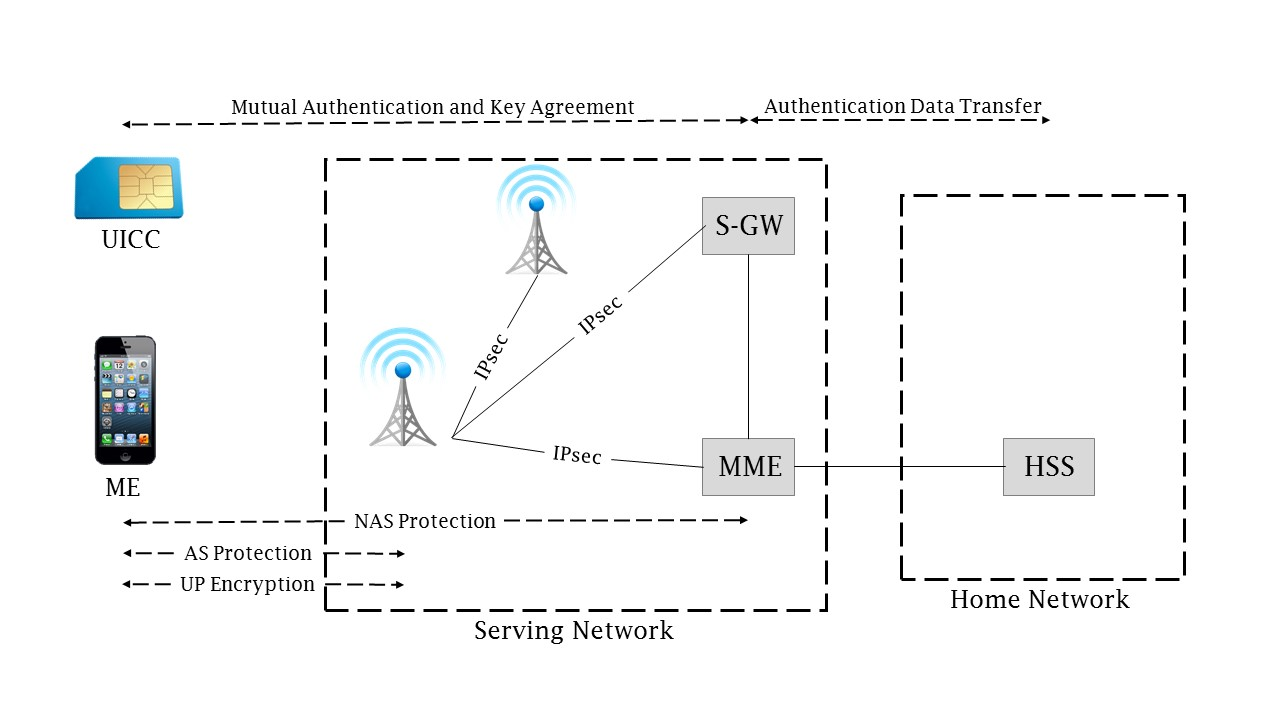
\includegraphics[width=1\linewidth]{architecture}
\hspace{0pt}
%\includegraphics[width=0.35\linewidth]{division}
\end{minipage} 
\end{center}

\section{Important facts about LTE/3G/GSM}
\begin{enumerate}
\item An ME connects to the base station in the vicinity that offers the strongest signal.
\item An ME identifies itself with the user's IMSI at the very first time it connects to a serving network (SN).
\item After the authentication and key agreement (AKA), the ME is given a temporary identity (TMSI) securely.
\item It is possible that either ME or SN loses TMSI causing the ME to remain out of the network.
\item To prevent from being kicked out of the network permanently, ME provides its IMSI in cleartext to any base station that asks for it.
\end{enumerate}


\section{IMSI catchers in LTE/3G/GSM}
It is a well known mechanism \citep{Ginzboorg_Niemi_2016}, \citep{ravi}.
\begin{enumerate}
\item IMSI catcher is a fake base station that impersonates a legitimate base station
\item The IMSI catcher offers strongest signal in the vicinity
\item All the users in the vicinity try to connect with the IMSI catcher since it offers the strongest signal
\item The IMSI catcher simply asks the identity of the ME user that tries to connect 
\item Every ME provides its user's IMSI in cleartext in response
\end{enumerate}


\begin{center}
\begin{minipage}[t]{0.3\linewidth} % logo
\vspace{0pt} % Alingns the parallel minipages on top
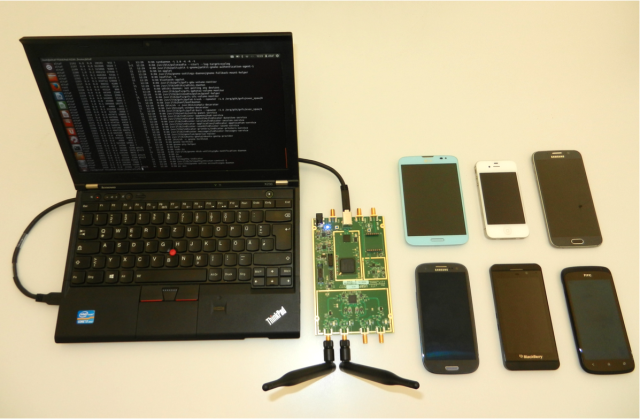
\includegraphics[height=0.6\linewidth]{imsicatcher}
\hspace{300pt}
%\includegraphics[width=0.35\linewidth]{division}
\end{minipage} 
\begin{minipage}[t]{0.33\linewidth} % logo
\vspace{0pt} % Alingns the parallel minipages on top
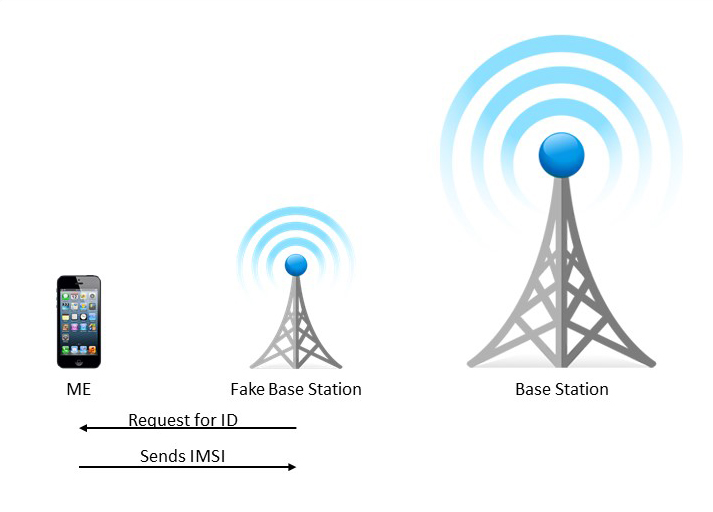
\includegraphics[height=0.6\linewidth]{imsicatcher1}
\hspace{0pt}
%\includegraphics[width=0.35\linewidth]{division}
\end{minipage} 
\begin{minipage}[t]{0.3\linewidth} % logo
\vspace{0pt} % Alingns the parallel minipages on top
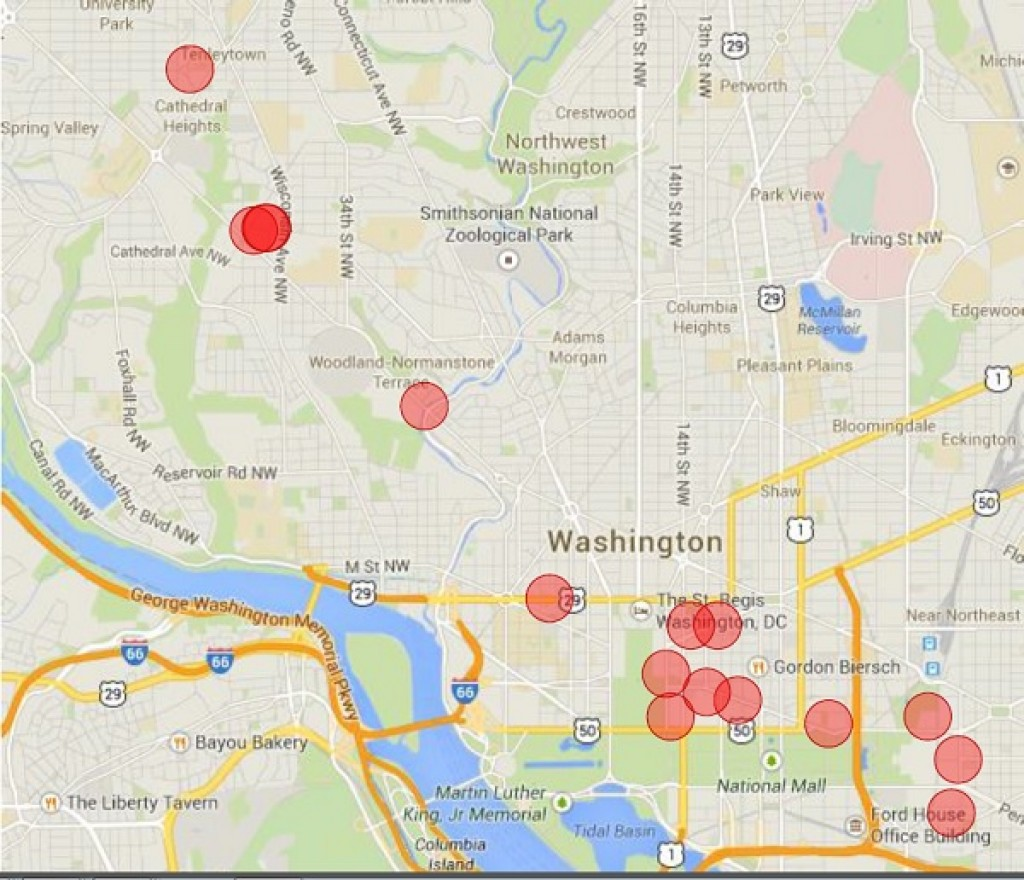
\includegraphics[width=0.6\linewidth]{mapnatsec}
\hspace{0pt}
%\includegraphics[width=0.35\linewidth]{division}
\end{minipage}
\newline
%\lipsum[1]
\end{center}

IMSI catching is not just a theoretical attack. The rightmost figure above shows how densely the IMSI-catchers existed in Washington in 2014 (Washington Post). To stop the IMSI catchers three different solutions have been published by researchers. 

%\section{How to stop IMSI catchers in 5G}
%Trivial solution is, never sending the IMSI in clear across the network. Researchers have come up two different approaches to tackle the problem. One is to encrypt the IMSI before sending across the network and the other is to use temporary identity called pseudonym as IMSI. The approach of encryption has the universal question of how to generate, exchange and manage the keys used for the encryption. Public-key and group-key have been proposed as potential solutions in this direction. The approach of pseudonym has the problem of keeping the mobile phone and home network (HN) in synch with the appropriate pseudonym.


\section{Solution 1: Public-key}
Solution with the public-key for every SN has the requirement of setting up a public key infrastructure (PKI) which is too expensive and hence has not been considered as feasible. However, solution with public-key for the HN is still a potential candidate \citep{Ginzboorg_Niemi_2016}.

\subsection*{Summary}
\begin{enumerate}
\item The ME encrypts the IMSI with the public key of HN and sends the ciphertext to HN via SN 
\item HN decrypts the ciphertext with its private key and reveals IMSI. 
\item HN generates and sends an authentication vector (AV) to the SN.
\item The AV is needed in an authentication and key agreement (AKA) protocol that runs in between ME and SN.
%\item SN and ME participate in an authentication and key agreement (AKA) protocol. AKA is a challenge-response based protocol. The challenge and expected response are mentioned in the AV.
%\item SN and UE runs AKA between them. SN also provides temporary identity for UE, which is to be used in all subsequent communications between SN and UE.
%\item In case of any connection lost, UE sends encrypted IMSI to start new session.
\end{enumerate}
\subsection*{Pros}
\begin{enumerate}
\item It doesn't require the ME and HN to be in any synchronized state. 
\end{enumerate}
\subsection*{Cons}
\begin{enumerate}
\item The public key ciphertexts are much longer than an IMSI. This causes exchange of longer messages during the AKA which is not compatible with legacy SNs. 
\item Extra computational load on the home subscription server (HSS) since public-key cryptography is computationally heavy
\item Increased latency
\end{enumerate}  

\section{Solution 2: Group-key}
\subsection*{Summary}
\begin{enumerate}
\item Every user belongs to a group in HN. Every group has a group-id and a group-key 
\item Group-id is a public information but the group-key is known only by HN and the users belonged to the group
\item When an ME connects to an SN, it encrypts the IMSI using the group-key and sends the encrypted IMSI along with the group-id
\item The SN forwards the encrypted IMSI and group-id to HN. 
\item HN resolves the group-key from the group-id and decrypt the IMSI
\item HN sends the IMSI the SN, together with AV that is needed for running the AKA procedure.
\end{enumerate}

\subsection*{Pros and Cons}
We have a trade-off situation for the size of the group \citep{Ginzboorg_Niemi_2016}:
\begin{enumerate}
\item If the group is too small, the group identity reveals too much about the user identity. For instance, it could be the case that only one member of the group is roaming in a certain country at a certain time point.
\item If the group is too large, then too many people would have access to the group key and the active attacker could be an insider from the group.
\end{enumerate}

\section{Solution 3: Pseudonym}
\begin{enumerate}
    \item  Every user having an IMSI is given a pseudonym $P$ by the HN initially.
    \item  When the user identifies itself with $P$ to the SN, the SN forwards $P$ to the HN
    \item In response, the HN sends a new pseudonym $P^{'}$ to the SN encrypted by the secret key $K$ or by some other secret key derived from $K$. The encrypted $P^{'}$ is embedded in the random challenge RAND that is needed for AKA.
    \item The SN runs the AKA with UE based on the AV. It also sends the encrypted new pseudonym $P^{'}$ to the UE.
    \item If the AKA is successful then the ME will be able to decrypt it and obtain $P^{'}$. The old pseudonym $P$ will be continued in use instead of IMSI until the UE tries to connect via another SN. 
    \item  When the UE tries to connect to the network via a new SN, the new SN has no knowledge about $P$. At this point instead of sending the IMSI, the UE identifies itself with $P^{'}$.
   % \item Whenever a new AKA is run, the HN generates a new pseudonym $P^{''}$ in the similar fashion mention in step \ref{scheme_aka_step}, replaces $P$ with $P^{'}$ and $P^{'}$ with $P^{''}$
\end{enumerate}
\subsection*{Pros}
\begin{enumerate}
\item Potentially compatible (if not readily) with legacy SNs and USIMs.
\end{enumerate}
\subsection*{Cons}
\begin{enumerate}
%\item We are critically attacking the solution to find and resolve weaknesses to make it compatible with legacy SNs and USIMs
\item It requires synchronized states in between ME and HN. Our research is currently focusing on this synchronization with minimal effort in the HSS. Currently our solution can generate an AV in at most $0.24$ milliseconds.
\item The size of the pseudonym space is only $10^{10}$. It seems the history of pseudonyms used has to be stored for a while because of billing. Storing this history will create some pressure on this space. We are working on estimating the pressure on this space and the usability of multiple MNC for a single operator to overcome the problem
\end{enumerate}

\section{Conclusions}
IMSI-catching is an attack that has existed though-out the history of cellular network. 3GPP focused on mitigating the attack during the design phase of GSM, 3G and LTE. But eventually no solution was adopted because of the added complexities they came with.  We have studied the aforementioned three solution candidates. We found the pseudonym approach to be the most appealing one because it has the opportunity to be implemented in 5G even when the SN is of from older generation.

\bibliographystyle{abbrvnat}
\bibliography{ref}

\end{multicols}

\vfill % some more marginal in the end

\begin{minipage}[t]{0.9\linewidth} % footer
\footnotesize
\color{gray}{\textsf{\textbf{The {\LaTeX} template by Jussi Tiira used in this poster is licensed under a Creative Commons Attribution 4.0 International License.}}}
\end{minipage}

\end{document}
